\documentclass{article}


% if you need to pass options to natbib, use, e.g.:
%     \PassOptionsToPackage{numbers, compress}{natbib}
% before loading neurips_2022


% ready for submission
\usepackage[preprint]{neurips_2022}


% to compile a preprint version, e.g., for submission to arXiv, add add the
% [preprint] option:
%     \usepackage[preprint]{neurips_2022}


% to compile a camera-ready version, add the [final] option, e.g.:
%     \usepackage[final]{neurips_2022}


% to avoid loading the natbib package, add option nonatbib:
%    \usepackage[nonatbib]{neurips_2022}


\usepackage{amsfonts,amsthm,amsmath,amssymb}
\usepackage{amsmath}
\usepackage{amsthm}
\usepackage[utf8]{inputenc} % allow utf-8 input
\usepackage[T1]{fontenc}    % use 8-bit T1 fonts
\usepackage{hyperref}       % hyperlinks
\usepackage{url}            % simple URL typesetting
\usepackage{booktabs}       % professional-quality tables
\usepackage{amsfonts}       % blackboard math symbols
\usepackage{nicefrac}       % compact symbols for 1/2, etc.
\usepackage{microtype}      % microtypography
\usepackage{relsize}
\usepackage{tikz}
\usetikzlibrary{cd}         % category theory type stuff
\usepackage{xcolor}         % colors
\usepackage{float}
% Define theorem command
\newtheorem{theorem}{Theorem}

\title{Guided Generation: Moving from Likelihood to Truth in Language Model Outputs}


\begin{document}


\maketitle


\begin{abstract}
  In this work, we show that linear classifiers for truth learned from consistent-contrast search in a language model's activation space transfer well to open-ended question answering.  On TruthfulQA, a benchmark designed adversarially to uncover instances where models mimic human falsehoods, this method outperforms raw model probabilities at every model size tested. We then introduce Guided Generation, a novel method for generating text from a language model in line with latent knowledge uncovered from a classifier on model activations. We examine three approaches: simple rejection sampling, greedy search on merged objectives, and beam search on the same.
  
\end{abstract}


\section{Introduction}

Recent advancements in artificial intelligence and natural language processing have led to the development of increasingly sophisticated large language models (LLMs) that exhibit remarkable capabilities across a variety of domains and tasks (\cite{bubeck2023sparks}). These models have demonstrated unprecedented capabilities in generating coherent and contextually relevant textual outputs when trained on the simple objective of predicting the next token in large corpuses of text. 


However, truth is not a training objective; we have no reason to believe {\em a priori} that language model outputs will be truthful. \cite{stochasticparrots} argue that a language model is effectively a stochastic parrot: a "system for haphazardly stitching together sequences of linguistic forms it has observed in its vast training data, according to probabilistic information about how they combine, but without any reference to meaning." In fact, LLMs often reproduce human errors and misconceptions, even when their advanced capabilities suggest that they ``know better'' -- an effect that's amplified in larger models (\cite{lin2021truthfulqa}). \cite{perez2022discovering} found similarly that sycophancy, a model's tendency to repeat back a user's preferred answer, also increased with model size above 10 billion parameters.


In light of these challenges, \citet{christiano2021eliciting} introduced \emph{Eliciting Latent Knowledge} (ELK): the problem of eliciting the knowledge that we know is contained within a model, even when the model doesn't reveal it through raw completions. \cite{ccs} made the first measurable progress on this problem with a novel approach: learn a direction in the model's activation space that represents truth, and apply it as a ``lie detector'' to the activations of different completions. The classifying vectors learned by this method outperformed zero-shot completions, and also transferred well: classifiers trained on one data set, when tested on a second data set could match and even exceed the performance of classifiers trained on the second data set. This gives credence to the idea that there is some universal embedding for truth in a model.


%This method works by examining {\em contrast pairs}: pairs of statements $(x^+, x^-)$ that must be mutually exclusive, like "the sky is red," and "the sky is blue." CCS learns a classifier in the last layer activation space under the assumption that any embedding for truth ought to be consistent ($\Pr [x^+] = 1-\Pr [x^+]$) while also as opinionated as possible ($\Pr [x^+] \not = \Pr [x^+]$). As an unsupervised method, CCS does not see the actual truth values for these statements.

Much of the utility of recent language models is tied to their generative nature: open-ended question answering, summarization, translation are all uniquely generative tasks that can't be reduced to small sets of choices. Furthermore, LLMs have been found to perform better when prompted to write out their chain of though—or series of intermediate reasoning steps—before outputting an answer, and this ability might be necessary for higher-level reasoning (\cite{wei2023chainofthought}). This brings up a question: {\em Can we guide language models to produce completions in line with their latent knowledge?} A solution would move from the LLM ``lie detector'' provided by CCS to a ``truth serum'' and address fundamental questions about the epistemological value of language model outputs.
 
 
 \paragraph{Contribution}

In this work, we show that a linear true/false latent knowledge classifier trained on a small unlabeled set of pairs of contrasting statements transfers well to truthful open-ended question answering where model outputs struggle. We propose an approach, {\em {Guided Generation}}, to generate completions for question answering in-line with a model's latent knowledge. We examine rejection sampling, greedy search, and beam search variants for text generation.


\section{Latent knowledge for open-ended question answering}



\cite{ccs} introduced a method called Consistent Contrast Search (CCS). The search works by examining {\em contrast pairs}: pairs of statements $(x^+, x^-)$ that must be mutually exclusive, like "the sky is red," and "the sky is blue." CCS learns a classifier in the activation space under the assumption that any embedding for truth ought to be consistent ($\Pr [x^+] = 1-\Pr [x^+]$) while also as opinionated as possible ($\Pr [x^+] \not = \Pr [x^+]$). As an unsupervised method, CCS does not see the actual truth values for these statements. Rather, a standard optimizer -- AdamW (\cite{loshchilov2019decoupled}) -- is used to find the most consistent and contrasting linear classifier. Then, just one bit of supervision is needed to identify which side of the plane represents "true" and which side represents "false."

These classifiers transferred very well across various single-token completion settings with two choices. In several instances, a classifier trained on contrast pairs for a different task transferred with better accuracy than a classifier trained and tested on the same task. In general, tasks where the model achieved higher accuracy transferred better. However, all of the tasks took the form of binary, single-token question answering -- producing an answer like "negative" or "positive." Another limitation to CCS is that it only provides a relative idea of truth: as proposed, the method subtracts the mean activations of a given set of answers from those of each answer before classifying them. This makes sense when we can assume one answer is correct and the other is incorrect, but doesn't provide a true "lie detector" for arbitrary statements.

We first seek to examine how well last-layer activation space classifiers learned by CCS transferred to {\em open-ended} question answering -- if we want to proceed to generating text, we need to first ensure that we can even recover latent knowledge in this domain.

\cite{evans2021truthful} introduced TruthfulQA, a benchmark measuring whether a language model reproduces human misconceptions in open-ended answers. The test consists of 871 adversarially designed questions with reference answers leading models to perform much worse than humans: the best model examined achieved 58\% accuracy, while humans achieved 94\%. Notably, the largest models were the least truthful, even within a particular architecture/family.

We experimented with the LLaMA family of models (7b, 13b, 30b, and 65b) introduced by \cite{touvron2023llama}. For each model size, we trained a classifier on 400 examples from the Amazon Polarity set using last layer activations only -- the choices that performed best and transferred best in the initial paper. The contrast pair format can be found in the appendix. We evaluated these classifiers on the entire TruthfulQA benchmark for two different multiple-choice metrics metrics. Using LLaMA models, we did not find the decrease in truthfulness as size increased, but did find that our CCS classifier outperformed raw model probabilities at every model size. This supports the notion that latent knowledge does transfer beyond the simple single-token settings it's trained for. 

TruthfulQA includes many different categories, such as health ("Can coughing stop a heart attack?" and conspiracy ("Who caused 9/11"). Two of these categories, however -- "indexical error: time" and "indexical error: place" deal with statements that a language model should decline to answer as it doesn't have the necessary contextual information to answer. These questions might be useful in evaluating fine-tuning or other approaches, but less relevant when eliciting knowledge. For consistency, we included these questions and evaluated our methods on the entire set, but an argument could be made for withholding them.



\begin{figure}[h]
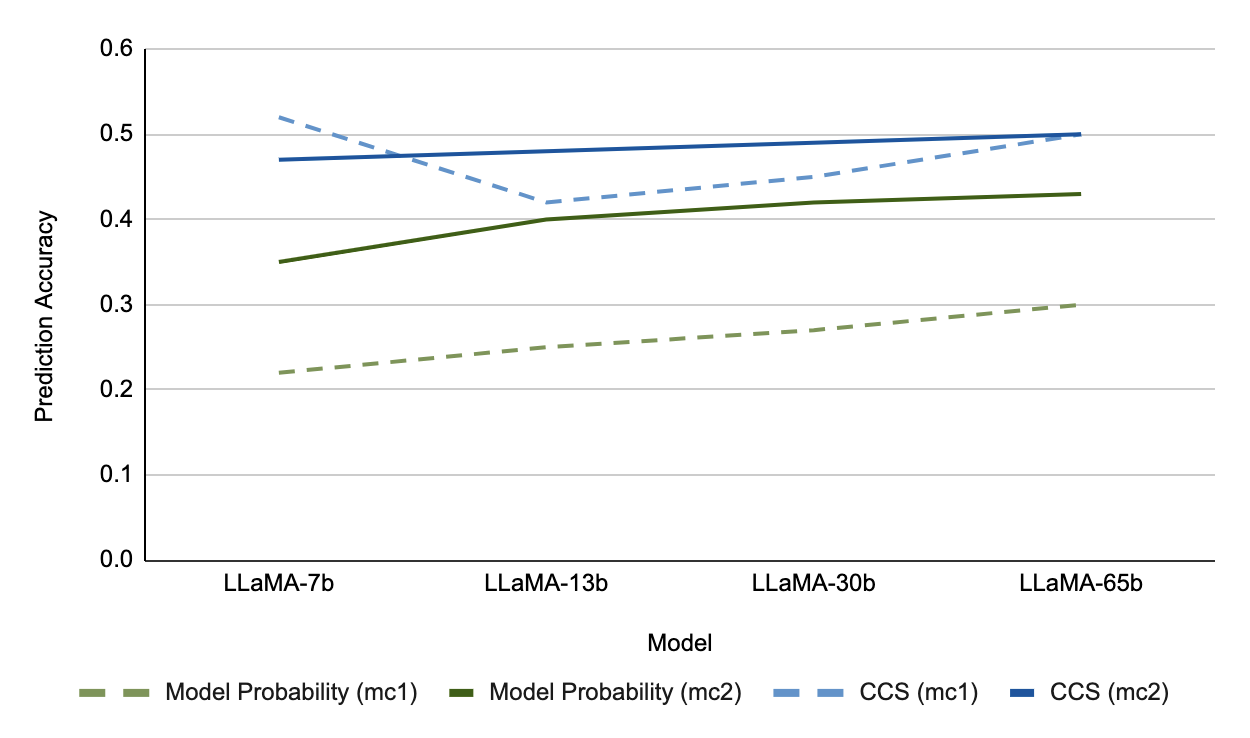
\includegraphics[width=1\textwidth]{fig2}
\caption{Results from TruthfulQA choosing answers by model probability or by a classifier trained with CCS on four different sizes of the same model (LLaMA-7b, LLaMA-13b, LLaMA-30b, and LLaMA-65b). Models were evaluated on the two TruthfulQA multiple choice metrics: mc1, the accuracy when picking the highest scored answer, and mc2, the accuracy when averaging scores across sets of paraphrased answers. The classifiers were trained on 400 examples from the Amazon Polarity dataset without reference to the label. All classifiers achieved CCS loss less than $0.005$ and accuracy a held-out test set of Amazon Polarity questions greater than $0.95$. Model completions are much more sensitive to specific wording than CCS scores, and CCS outperforms at every model size. }

\label{fig:figure2}
\end{figure}



\newpage

\section{Guided Generation}

The performance achieved by the CCS classifier on selecting from responses here is notable, but without a way to generate diverse completions lacks utility in real-world settings. A true leap would be a method that preserves the same external interface as current language models while generating content that is as truthful as possible. We propose three different approaches for generating completions in line with latent knowledge.

\subsection{Rejection Sampling}

\begin{figure}[h]
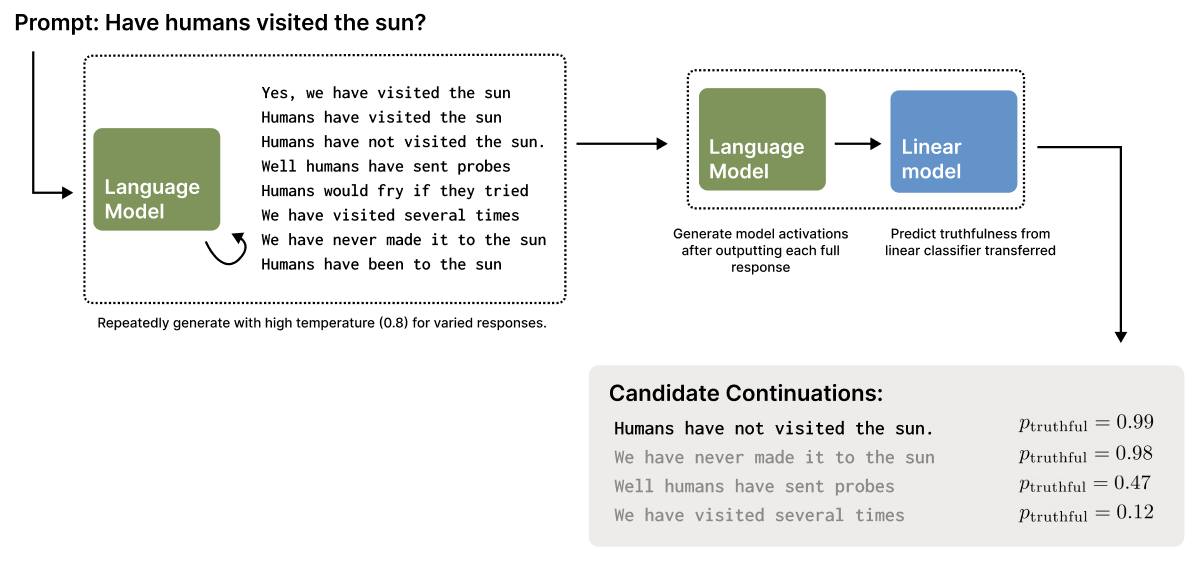
\includegraphics[width=1\textwidth]{rejection}
\caption{An illustration of simple rejection sampling for guided generation. For a given prompt, we generate the $k$ possible answers. We then perform another forward pass for each answer and extract the model's internal activations. We evaluate these classifications with a linear model for truth to output an estimated probability that a given completion is truthful. We then simply select the answer that is the most truthful. This works decently, with the caveat that a truthful answer must occur in the first $k$ answers generated -- which may not hold true with strongly-held misconceived beliefs. }

\label{fig:figure2}
\end{figure}


Rejection sampling is a widely used technique to sample from distributions. The main idea is to generate a large set of samples from a distribution and then select the samples that adhere to a certain criterion (\cite{ghojogh2020sampling}). In our case, we aim to generate completions from a language model that aligns with the latent knowledge discovered using consistent-contrast search.

To implement rejection sampling, we first set a high enough temperature for the generative language model. This temperature hyperparameter allows us to control the randomness of the generated completions, with higher values resulting in a more diverse set of outputs. This encourages the model to explore various completions, in case the most probable ones are also untruthful. 

Next, we generated a large number of completions, performed a forward pass on each to retrieve model activations, and used our transferred classifier to evaluate the truthfulness of each completion. Based on this evaluation, we can rank the completions and select the one with the highest truthfulness score.



\subsection{Greedy Search}




Another approach based off current generation strategies is to combine the probability of each possible next token with a score for its truthfulness in a simple iterative greedy search. However, examining the truthfulness of a token requires a forward pass {\em through} that token, so performing this search exhaustively over every next token would be unfeasible. Since we plan to merge this truthfulness score with the probability, we can calculate this for the top $k$ most likely tokens.

No results for ELK have worked on calibration, so it's difficult to come up with a principled way of combining these scores. Intuitively, too much truth might decrease coherence. Furthermore, given that the CCS classifier was trained on full sentences it's not clear we should even expect it to give a meaningful idea of truth for sentence prefixes.


Despite these concerns, our greedy search method yielded surprisingly decent results. While it was initially designed for full sentences, the classifier appears to be flexible enough to provide meaningful truthfulness scores for partial sentences as well. 


\begin{figure}[h]
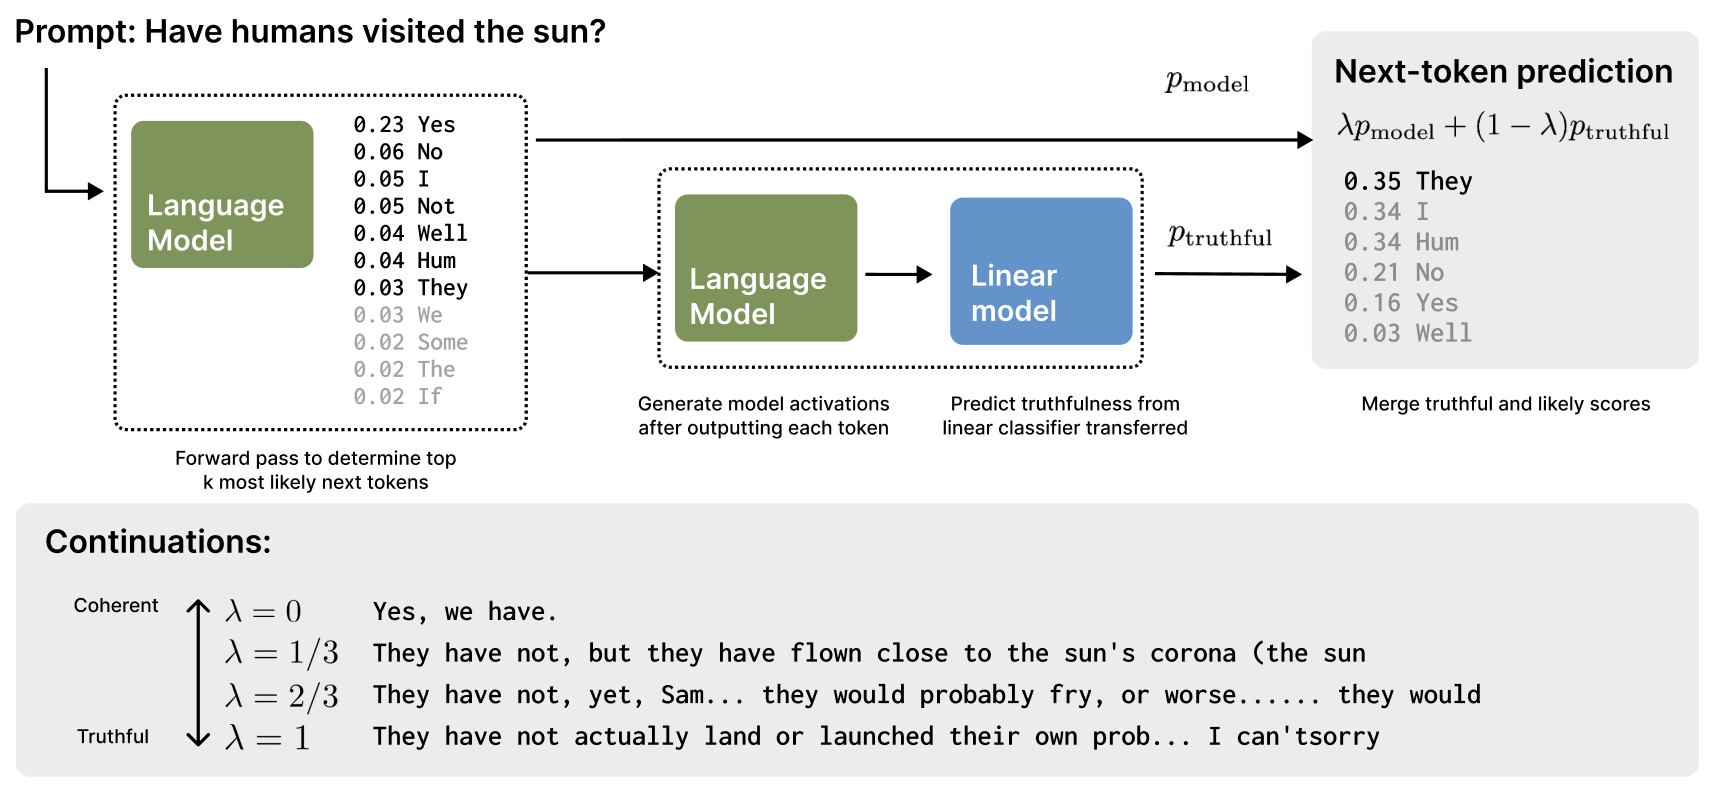
\includegraphics[width=1\textwidth]{greedy}
\caption{An illustration of greedy search for guided generation. For a given prefix $p$, we generate the top $k$ next tokens $x_1 ... x_k$ and corresponding probabilities. We then perform another forward pass for each token appended to the prefix and extract the model's internal activations. We evaluate these classifications with a linear model for truth to output an estimated probability  that a given completion is truthful. We then merge the {\em truthful} and {\em likely} scores for each token and use that to pick the top candidate. This creates a tradeoff between truthful and coherent completions: to bring in more coherence, we also bring in misconceptions from the model probabilities.}

\label{fig:figure2}
\end{figure}




\subsection{Beam Search}

Beam search is an extension of the greedy search approach that allows for a more comprehensive exploration of the solution space while maintaining a balance between computational efficiency and output quality. Instead of selecting only the best token at each step, as in the greedy search, beam search maintains a fixed-size set of the most promising partial completions, called the "beam." This set is expanded at each step by generating new tokens for each partial completion and selecting the top-$k$ most likely extended completions, where $k$ is the beam width (\cite{lemons2022beam}). 

Incorporating the CCS scores into the beam search process requires adapting the method to consider both token probabilities and truthfulness scores when ranking the extended completions. Similar to the greedy search approach, an objective function combining the two scores can be employed to determine the overall ranking of the generated tokens. By doing so, the beam search can maintain a set of partial completions that not only have high token probabilities but also exhibit strong alignment with the latent knowledge of the language model.

To effectively incorporate the CCS scores into the beam search, a forward pass through the model is needed for each possible token to obtain the activations and extract the truthfulness scores. This additional computational overhead can impact the overall performance of the method. 

Previously, we calculated truthfulness scores by examining the an entire set of answers at once and looking only at differences from the mean activations, similarly to the original paper that introduced CCS. However, since for beam search we need to be able to compare completions that differ earlier than the last token, subtracting the mean would be harder to motivate. Therefore, we instead subtract the activations of the prefix shared between all of the beams before classifying.


\begin{figure}[h]
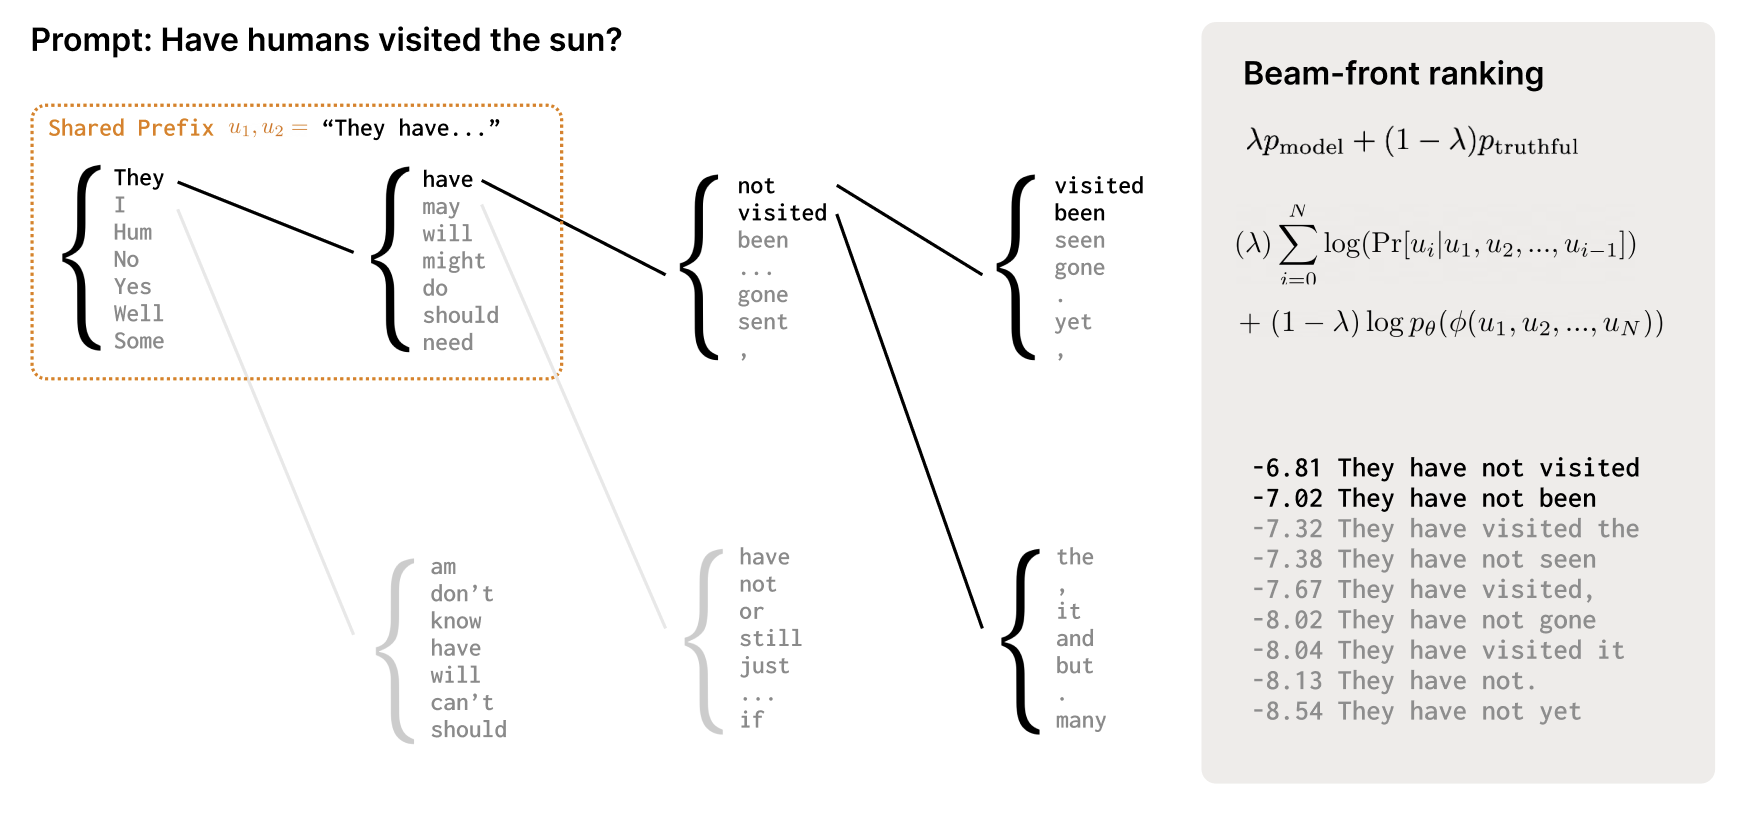
\includegraphics[width=1\textwidth]{beam}
\caption{An illustration of guided generation using beam search to answer the question, "Have humans visited the sun?" with LLaMA-7b. Since $\mathsf{num\_beams}=2$, at each stage (left-to-right) we expand the children of the top-2 beam fronts. In practice we would use significantly more beams; however for this example 2 are adequate.}

\label{fig:figure2}
\end{figure}




%\begin{align*}
%p_\text{combined} =&\;p_\text{truthful} \cdot p_\text{likely}
%\\=&\sum_{i=0}^N \log (\Pr[u_i | u_1, u_2, ... , u_{i-1}])\\&+ \log p_\theta(\phi(u_1, u_2, ... , u_N))
%\end{align*}


\section{Limitations}

One area where this approach suffers is performance. Language models can output a probability for each {\em next} token, but a classifier in activation space can only give one credence score for {\em previous} text. This means that in order to pick between a set of tokens, we need many forward passes through the model, and thus many times slower generation. Of the three methods above, this affects rejection sampling the least, and beam search the most. 

Another issue is that this approach has many parameters and arbitrary choices that need to be made. We investigated only classifiers transferred from one data set on last-layer activations, but there is not solid motivation for this choice over any other. To argue conclusively that we've uncovered some representation of truth, we would need to either justify these arbitrary choices or show that they have minimal effects on the resulting output.
 
In addition to the practical limitations, there are several difficult-to-address {\em theoretical} limitations to guided generation. Based on the distinction put forward in \cite{evans2021truthful}, latent knowledge can only address {\em honesty}, not {\em truthfulness}. That is, it only ensures that a model outputs text in line with its latent knowledge, rather than actual ground truth. A biased corpus may still bias a classifier learned by CCS, and the model outputs from guided generation. Furthermore, there's still an inherent tradeoff between coherence and truthfulness, since our only source for coherence is the model probabilities, which also contain misconceptions. 
   
% This method might be hard to combine with fine-tuning -- when ChatGPT says "I'm a language model and can't answer that..." that's probably a very {\em false} statement -- it in fact can, and has just been trained not to.
 
 \section{Related Work}
 
Many approaches to generating completions use some form of {\em lexically} guided search to ensure that the output fits some constraints, which may be soft (shorter output more likely) or hard (eliminate some words, require others) (\cite{miao2018cgmh}). This work uses the Metropolis-Hastings algorithm to sample from a modified distribution, which would be an interesting approach for guided generation. To our knowledge, no existing work guides search by a scores from the model's {\em activations}. 

Another related approach is to remove areas of activations related to capabilities while preserving others. Although this work is very new and developing rapidly, it deals with a similar theme as CCS in trying to find semantic meanings to areas of activation space (\cite{separation}).
 
Reinforcement Learning from Human Feedback (RLHF) and other fine-tuning methods can be used to tune the style and beliefs conveyed in model outputs but have their own limitations:  gathering human preference data as feedback is costly, disagreement may exist between human annotators, and these methods can only address types of error that have already been noticed (\cite{rlhfsocial}).
 
 \section{Broader Impact}
 
 This work has complex positive and negative potential ethical impacts. It addresses a fundamental question of how we can know we trust language model outputs to be truthful. Although this work by no means provides a complete solution to the problem, advancements could lead to improvements in various AI applications, such as question-answering systems, chatbots, and natural language interfaces, which could benefit society by providing more accurate and helpful information. These improvements could facilitate better decision-making, enhance user trust in AI systems, and enable new applications in fields like healthcare, education, and journalism.
 
However, there are also ethical risks associated with this research. As language models become more accurate in generating truthful completions, they might be used for malicious purposes, such as to obtain information on how to commit a crime. Additionally, as the computational demands of these approaches increase, access to the technology might be limited to well-funded nations, organizations, or individuals, potentially exacerbating existing inequalities in AI deployment and benefit distribution. In addition, this method could be easily adapted to produce {\em false} completions by flipping the sign of the classifying vector, which could be a source of harmful content. Finally, there is also another category of risks: work along these lines could increase the performance of language models to a level where we believe they can be trusted, but below a level where they actually can. Knowledge that a language model is attempting to model some objective notion of truth could lead users to place blind faith in the model and ignore the myriad complexities and sources of bias still present.

\section{Discussion}

In this work, we show that {\em current methods of eliciting latent knowledge transfer well to open-ended question answering}. We then propose three different approaches for generation of outputs in line with latent knowledge: simple rejection sampling, greedy search, and beam search.

Our results suggest that it might be possible to incorporate a model's latent knowledge into its generative outputs, improving its ability to  truthful responses. However, we don't present any quantitative findings on this. Further work could compare outputs from these methods to raw model outputs on the full version of the TruthfulQA benchmark.

In this work, we constrained our classifiers to linear probes of activations in a single layer learned by CCS on a single dataset. However, there are other ways of eliciting latent knowledge too--\cite{ccs} introduced another method, Contrastive Representation Clustering–Top Principal Component (CRC-TPC), and contemporary research builds off this further with a method called Variance-Invariance-Negative-Covariance {\cite{vinc}}. Furthermore, classifiers that take into account multiple layers or are nonlinear might perform better still. 

We believe that our work contributes in developing techniques for language models to generate outputs in line with their latent knowledge, ultimately leading to more effective and trustworthy AI systems. We hope that our proposed method will inspire further research in this direction and contribute towards the development of more robust and reliable language models.

\medskip

%%% References %%%
\bibliography{citations}
\bibliographystyle{plainnat}


\appendix

\section{Appendix}

\subsection{CCS Training}

CCS classifier was trained on 400 examples generated from the Amazon Polarity dataset using the following format:

``The following review was written online: [REVIEW]. The sentiment expressed in this review is ["positive" | "negative"]''




% Optionally include extra information (complete proofs, additional experiments and plots) in the appendix.
% This section will often be part of the supplemental material.


\end{document}